В процессе взаимодействия клиентов с информационным центром возможно:
\begin{enumerate}
	\item режим нормального обслуживания, т.е. клиент выбирает одного из свободных операторов, отдавая предпочтение тому у которого меньше номер;
	\item режим отказа в обслуживании клиента, когда все операторы заняты.
\end{enumerate}

\textbf{Переменные и уравнения имитационной модели}  

\textbf{Эндогенные переменные}: время обработки задания i-ым оператором, время решения этого задания j-ым компьютером.

\textbf{Экзогенные переменные}: число обслуженных клиентов и число клиентов, получивших отказ.

Структурная схема представлена на рисунке \ref{fig2:image}, на нем К1-К3 моделируют работу операторов, К4-К5 -- компьютеров.
\begin{figure}[h]
	\begin{center}
		{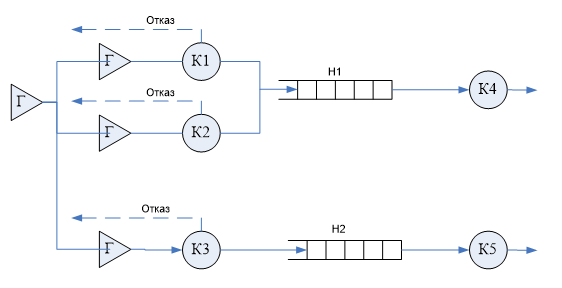
\includegraphics[scale = 0.9]{img/struct.png}}
		\caption{Структурная схема}
		\label{fig2:image}
	\end{center}
\end{figure}

